
%(BEGIN_QUESTION)
% Copyright 2006, Tony R. Kuphaldt, released under the Creative Commons Attribution License (v 1.0)
% This means you may do almost anything with this work of mine, so long as you give me proper credit

$$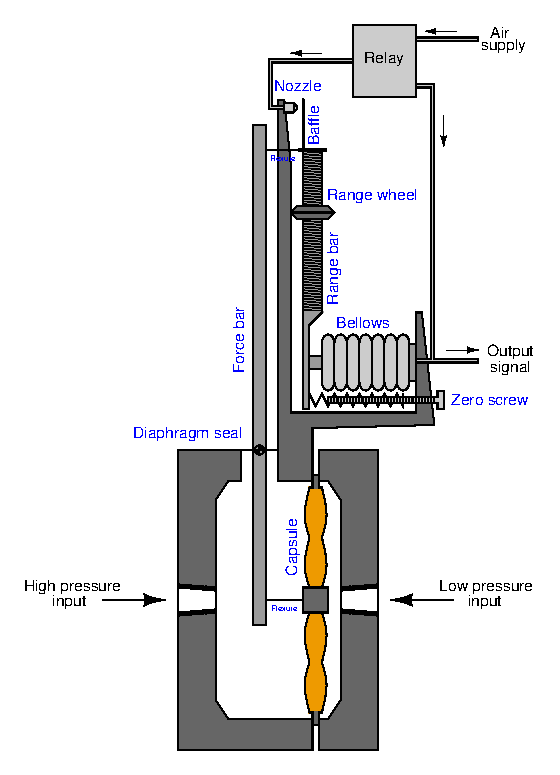
\includegraphics[width=15.5cm]{i00025x01.eps}$$

Skisser en pil som viser hvilken retning {\it range wheel} må flyttes for å øke transmitterens målespenn (dvs. slik at 3-15 PSI ut representerer et {\it større} spenn av prosesstrykk enn før).

\vskip 10pt

Skisser en pil som viser kraftretningen som påføres av {\it zero screw} på {\it range bar} for å øke utgangstrykket når ingen prosesstrykk er påført transmitteren (f.eks. 3.1 PSI i stedet for 3.0 PSI ved 0 PSID inngang).

\vfil 

\underbar{file i00025}
\eject
%(END_QUESTION)





%(BEGIN_ANSWER)

Dette er et vurdert spørsmål -- ingen svar eller hint gis!

%(END_ANSWER)





%(BEGIN_NOTES)

$$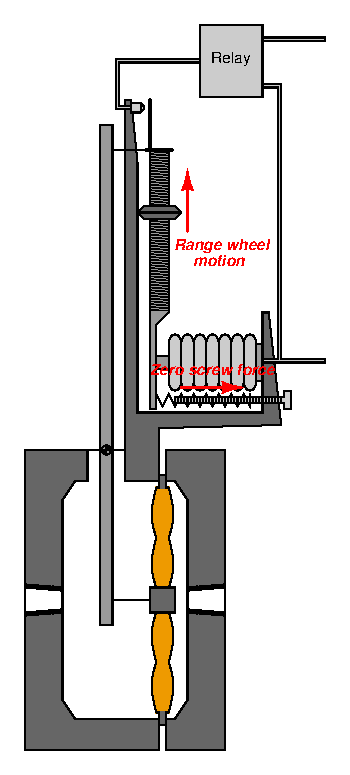
\includegraphics[width=15.5cm]{i00025x02.eps}$$

For å få 3-15 PSI til å representere et større spenn av prosesstrykk, må vi gi kapselen en ulempe og belgen en fordel.  Med andre ord må vi kalibrere transmitteren slik at kapselen må "jobbe hardere" for å fremkalle samme 3-15 PSI pneumatiske utgang -- kapselkraften må øke samtidig som den balanserer samme belgkraft.  Siden dette er et kraftbalanseinstrument, betyr det å gi kapselen den {\it kortere} enden av spaken og belgen den {\it lengre} enden av spaken.  Løsningen er derfor å flytte range wheel opp.

\vskip 10pt

For å forskyve 3-15 PSI-området oppover til 3.1-15.1 PSI må vi justere mekanismen slik at det er mer bias-kraft fra nullfjæren enn før.  Det vil si at belgen må "jobbe hardere" (gi mer kraft) for å holde likevekt uten påført trykk på kapselen.  Dette betyr at vi må trekke mer i nullfjæren enn før, slik at belgen må presse tilbake på range bar med større kraft.

%INDEX% Illustration, Foxboro 13A DP cell
%INDEX% Measurement, pressure: pneumatic DP transmitter

%(END_NOTES)
